\subsection{Methane decomposition using a hydroxyapatite supported nickel catalyst.}%
\label{sub:methane_decomposition_using_a_hydroxyapatite_supported_nickel_catalyst_}
One method of methane decomposition currently relies on a nickel catalyst, supported by compounds such as \ce{TiO2}, \ce{MgO}, \ce{ZrO2} and \ce{Al2O3}.
The rate of reaction depends on the \ce{Ni} particle size, with both relation to the dispersion and stabilisation by a suitable support\cite{Ashok}.
J. Ashok et al. have been looking at a new nickel catalyst support, hydroxyapatite (\ce{HAp}), and how it will affect this reaction.

 \ce{HAp} is produced from a reaction of \ce{Ca(NO3)2.4H2O} and \ce{(NH4)2(PO3OH)} to make \ce{[Ca5(PO4)3(OH)]} while under basic conditions\cite{Ashok}.
Unlike the previously mentioned catalyst supports, \ce{HAp} is irreducible; this means there is no \ce{CO} made in the reaction unlike the other catalyst supports currently in use.
This means the reaction has a simple overall equation with no greenhouse gas (GHG) emissions:
\begin{align}
	\ce{CH4 -> C +2H2}
.\end{align}
This reaction has an enthalpy of \SI{75.6}{\kilo\joule\per\mole} meaning it is endothermic.
The experiment was run at just \SI{650}{\celsius}\cite{Ashok}, which is a mild reaction condition for an endothermic process.
The \ce{CH4} should be flowed through the reaction chamber at a slow \SI{24}{\liter\per\hour}\cite{Ashok} again meaning no extra energy is needed to accelerate the gas.
These combined factors and the lack of GHGs produced make this reaction both green and sustainable.

\begin{figure}[H]
	\centering
	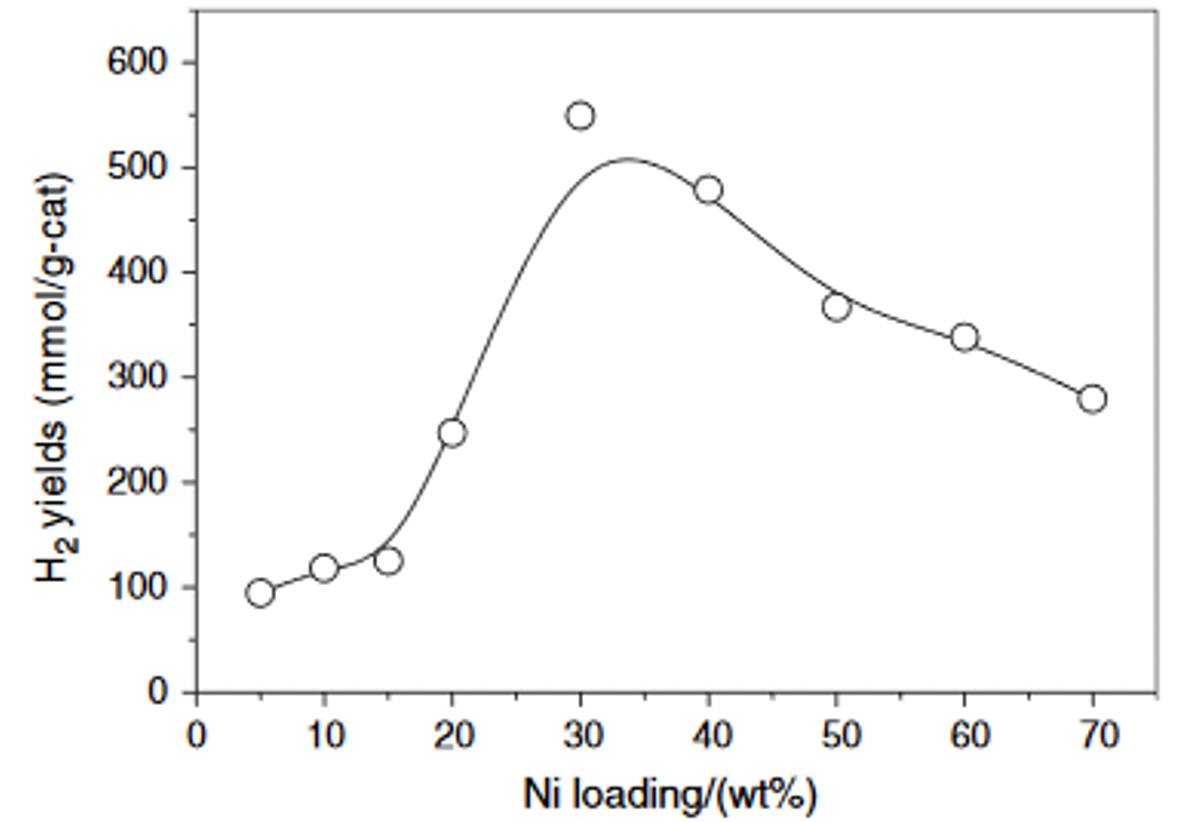
\includegraphics[width=0.4\textwidth]{539a7840-2cb8-11eb-895f-8c8590753a48.png}
	\caption{A plot of percent weight of nickel loaded onto the catalyst support vs \ce{H2} yield.}  
	\label{fig:MD_plot1}
\end{figure}

\begin{figure}[H]
	\centering
	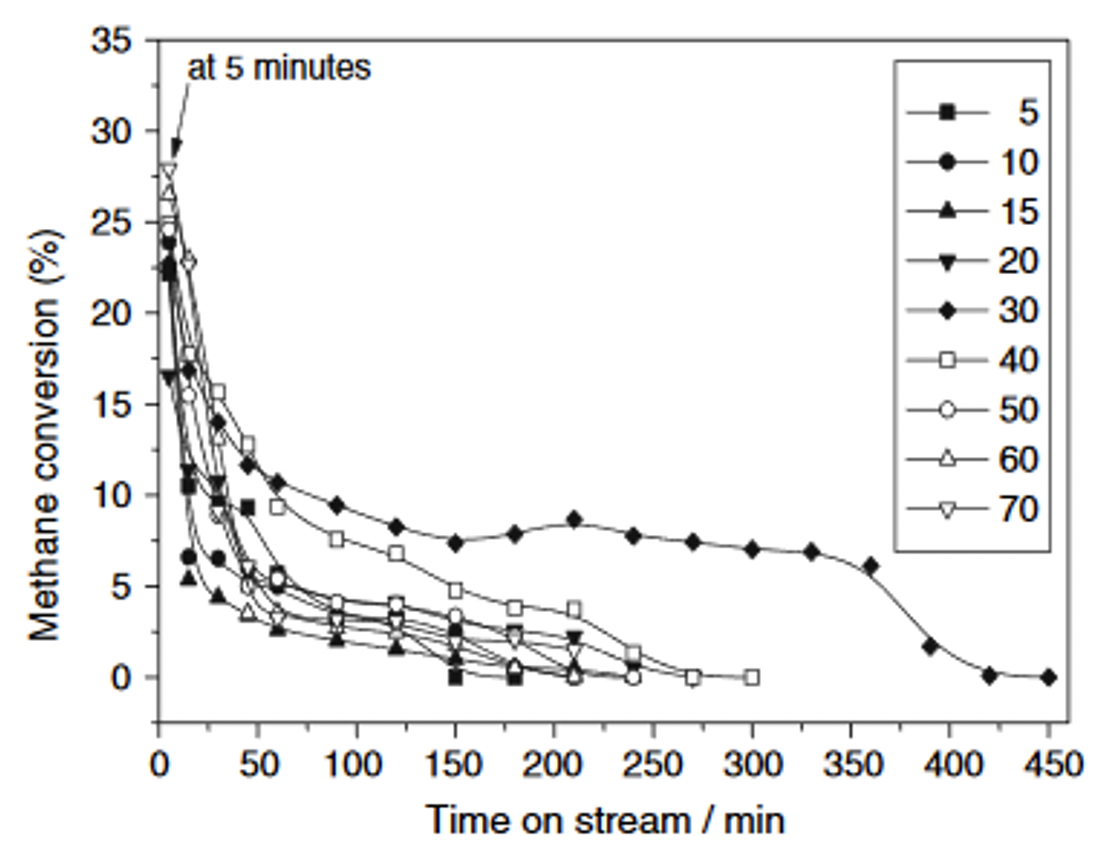
\includegraphics[width=0.4\textwidth]{0ed19cac-2cb8-11eb-895f-8c8590753a48.png}
	\caption{A multiple plot of varying percent weights of nickel loaded onto the support showing how methane conversion efficiency varies with time.}
	\label{fig:MD_plot2}
\end{figure}

As you can see from figures \ref{fig:MD_plot1} and \ref{fig:MD_plot2} a 30 wt\% \ce{Ni} sample was the optimum for this reaction.
It has both the highest yield and the best durability.
This reaction does have one major drawback however in that the catalyst readily degrades.
This means the solid waste carbon, which is responsible for the deactivation of the catalyst, will be contaminated with toxic \ce{Ni} atoms.
This is a very promising technology which warrants further research, as it can help to solve the current \ce{H2} crisis.


\subsection{Radical methane pyrolysis}%
\label{sub:radical_methane_pyrolysis}
Radical methane pyrolysis (RMP) is a way of breaking a \ce{CH4} molecule into \ce{H2} and pure carbon.
The initial step is the chemisorption of \ce{CH4}, onto the surface of the catalyst.

\begin{align}
	\intertext{The initiation and rate determining step of the radical breakdown is:}
	\ce{CH4&-> ^.CH3 + H^.}
	\intertext{Then a series of propagation steps take place with the general equation:}
	\ce{^.CH_{n}&-> ^.CH_{n-1} + H^.}
	\intertext{Until a termination step is reached:}
	\ce{4H^.&-> 2H2}
	\intertext{This gives the overall equation of:}
	\ce{CH4&-> C + 2H2} \label{eq:RMP_rct}
.\end{align}

This reaction \eqref{eq:RMP_rct} gives rise to no waste gases such as \ce{CO2}, but does have the issue of elemental carbon production which can lead to the degradation of the catalyst as carbon is deposited upon the catalyst surface.
The reaction conditions for this mechanism follow Le Chatelier’s principle.
The reaction is endothermic with an enthalpy of reaction ($\Delta_{r}H$) of \SI{+37.5}{\kilo\joule\per\mole} which is very low when compared to electrolysis which has an $\Delta_{r}H$ of \SI{+286}{\kilo\joule\per\mole}\cite{SBN2020}.
Due to the endothermic nature of the reaction a high temperature is needed; as there are more moles on the RHS, low pressure is needed.
This is very expensive to maintain.
The methane should also move at a low velocity as this increases the contact efficiency between the methane and the catalyst, this results in a higher quantity of methane being adsorbed on the active site of the catalyst which means the catalyst will deteriorate more slowly.

Various metal or carbon-based catalysts can be used.
The main catalysts in a metal catalysed reaction are nickel and iron, these are particularly useful as partially filled \ce{3d} orbitals accept electron density from the \ce{CH} bonds, destabilising their bond strength and ultimately leading to the breaking of the bond.
These metals allow carbon diffusion through the crystalline structure.
Table 1 shows a few key aspects of the catalysts including how they affect the operating conditions and the overall reaction process.

%\end{multicols}
\begin{table}[H]
	\centering
	\caption{Catalytic efficacies, all relative values are compared to nickel.}
	\label{tab:catTab}
	\resizebox{\columnwidth}{!}{%
		\begin{tabular}{|l|l|l|l|l|l|}
		\hline
		Catalyst & Rate & Toxicity & Cost & Durability & \wrap{Operating temperature(\si{\celsius})}\\
		\hline	
		Nickel & Equal & Equal & Equal & Equal & $500-700$ \\
		Iron & Low & Low & Low & High & $700-1000$ \\
		Carbon & Low & - & Low & High &  $800-1000$ \\
		None & Very Low & - & - & - &  $1100-1200$\\
		\hline
		\end{tabular}
	}
\end{table}
%\begin{multicols}{2}

\ce{Ni} while an effective catalyst, has a major drawback compared to the other catalysts available; its toxicity results in the waste carbon being contaminated with \ce{Ni} catalyst.
 
\ce{Fe} catalytic activity is lower than that of \ce{Ni} however it is more resistant to catalytic deactivation.
This is because carbon has a higher rate of diffusion in \ce{Fe}, meaning it does not deposit itself upon the active site of the catalyst.
It also has the advantage of being able to operate at high temperatures in the range of \SIrange{700}{1000}{\celsius} and it is both cheaper and less toxic than \ce{Ni}.
\ce{Fe} compounds such as \ce{[Fe(CO)5]}, \ce{[Fe(cp)2]} have been tested as catalysts.

However, these types of iron clusters can result in unwanted gases, meaning the \ce{H2} has to be separated from the gaseous mixture, decreasing the reaction efficiency.
A catalyst with a strong support increases the carbon dispersion and reducibility of the metal along with preventing sintering of metal particles.
However, an excessively strong support may hamper the reducibility of metal oxides.
A supported catalyst has a better performance as it balances the carbon dispersion resulting in a longer lasting catalyst, while maintaining the reducibility of the metal species.

There are three types of carbon catalyst; highly ordered, less ordered, and disordered.
Disordered carbon catalysts have free valence sites or uncoordinated sites, known as high energy sites (HES).
The more HESs there are the faster the rate as these are thought to initiate the mechanism.
More oxygenated catalysts have a higher activity but release \ce{COx}, this is because as \ce{COx} is produced new active sites are created on the surface of the catalyst.
RMP is a very promising new piece of technology that combines both new and old science.
We believe that RMP with an \ce{Fe} catalyst will go a long way to solve the \ce{H2} problem.

\subsection{Discussion of methane methods}%
\label{sub:discussion_of_methane_methods}
Currently SMR provides around \SI{48}{\percent} of the worlds \ce{H2}\cite{SBN2020}, but this could soon change.
With the development of new reactions and catalysts, new and sustainable methods of \ce{H2} production from methane are on the rise.

\begin{figure}[H]
	\centering
	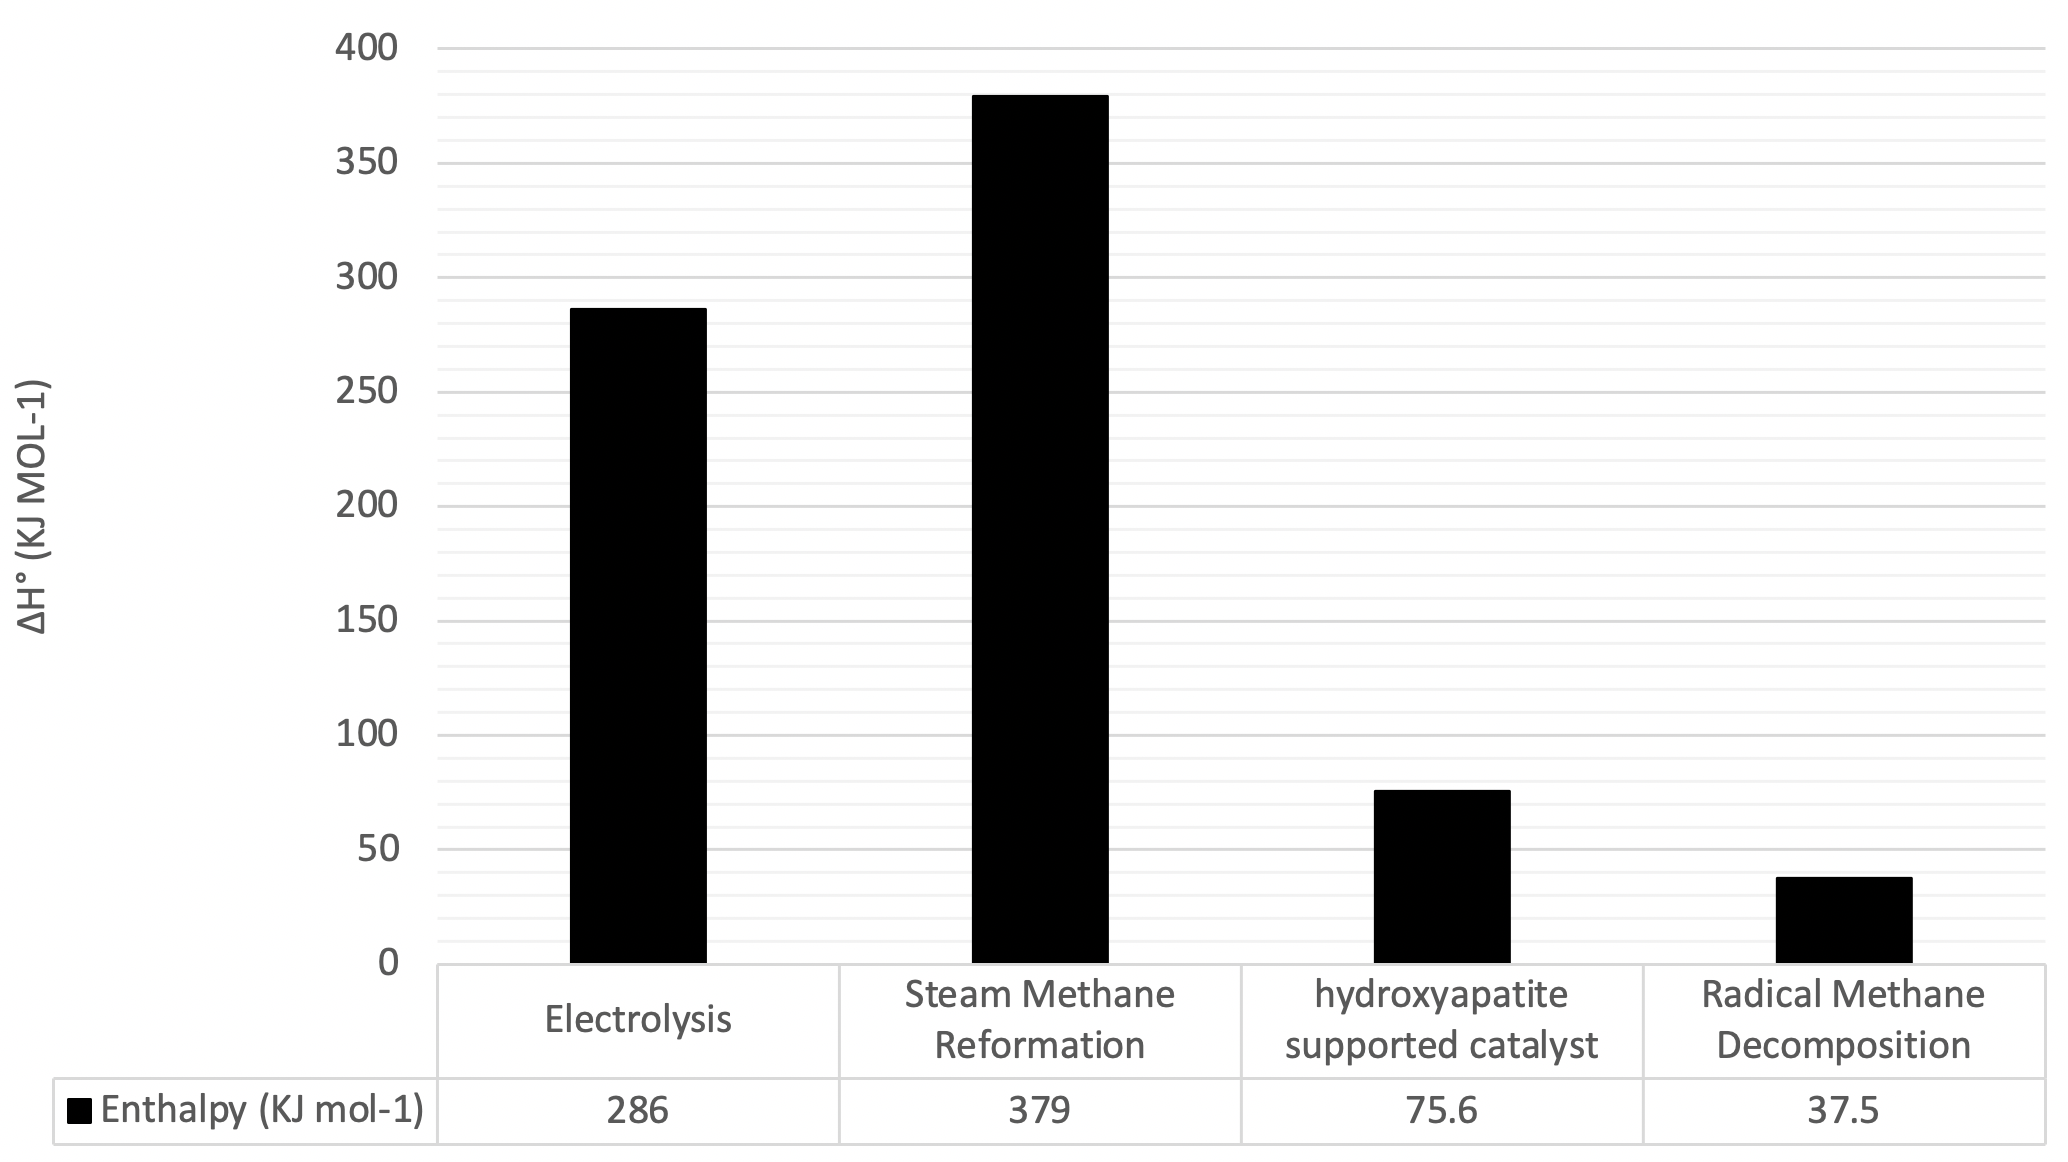
\includegraphics[width=0.4\textwidth]{6b76c760-2cb9-11eb-895f-8c8590753a48.png}
	\caption{A plot showing the enthalpy of the three methane methods alongside uncatalyzed electrolysis as a reference.\cite{SBN2020,Ashok,Saxena2011}}
	\label{fig:ME_disc}
\end{figure}

As you can see from figure \ref{fig:ME_disc}, radical methane decomposition and hydroxyapatite supported \ce{Ni} catalysts have a significantly lower enthalpy cost meaning they are far more economical processes.

Both \ce{HAp} and RMP both run at much lower operating conditions compared to SMR, this is beneficial not only to the cost of the reaction, but also to the greenness and sustainability.
Further aiding their sustainability is the lack of GHGs produced by both new reactions.
As there are no GHGs produced in either method, no separation step is required to extract the \ce{H2} gas, another positive when compared to SMR.

There are however drawbacks to the new methods of production.
The carbon byproduct is not resellable for three reasons: there is no market for it, the carbon rapidly degrades the catalysts and where \ce{Ni} catalysts have been used, the carbon is contaminated with toxic metal\cite{sbn2020}.

Therefore RMP has been shown to be a superior method to \ce{HAp}.
RMP has the option of using carbon or iron catalysts instead of nickel whereas \ce{HAp} only uses toxic nickel catalysts.
The carbon catalysts have a longer life than metals and also run at lower temperatures.
